\mode*
\lecture[proc]{proc}{proc}

\section{Processes}

\subsection{Processes, Lightweight Processes, and Threads}

\begin{frame}{Processes}
  \begin{description}
  \item[A process] is
    \begin{itemize}
    \item an instance of a program in execution
    \item a dynamic entity (has lifetime)
    \item a collection of data structures describing the execution progress
    \item the unit of system resources allocation
    \end{itemize}
  \end{description}
  The Linux kernel internally refers to processes as \textcolor{blue}{\emph{tasks}}.
\end{frame}

\begin{frame}{When A Process Is created}
  The child
  \begin{itemize}
  \item is almost identical to the parent
    \begin{itemize}
    \item has a logical copy of the parent's address space
    \item executes the same code
    \end{itemize}
  \item has its own data (stack and heap)
  \end{itemize}
\end{frame}

\begin{frame}{Multithreaded Applications}
  \begin{block}{Threads}
    \begin{itemize}
    \item are execution flows of a process
    \item share a large portion of the application data structures
    \end{itemize}
  \end{block}
  \begin{block}{Lightweight processes (LWP) --- Linux way of multithreaded
      applications}
    \begin{itemize}
    \item each LWP is scheduled individually by the kernel
      \begin{itemize}
      \item no nonblocking syscall is needed
      \end{itemize}
    \item LWPs may share some resources, like the address space, the
      open files, and so on.
    \end{itemize}
  \end{block}
\end{frame}

\subsection{Process Descriptor}

\begin{frame}{Process Descriptor}
  To manage processes, the kernel must have a clear picture of what each process is doing.
  \begin{itemize}
  \item the process's priority
  \item running or blocked
  \item its address space
  \item files it opened
  \item ...
  \end{itemize}
  \begin{description}
  \item[Process descriptor:] a \texttt{task\_struct} type structure containing
    all the information related to a single process.
  \end{description}
  \begin{center}
    \mode<beamer>{ \includegraphics[width=.7\textwidth]{task-struct2} }
    \mode<article>{ \includegraphics[width=.4\textwidth]{task-struct2} }
  \end{center}
\end{frame}

\subsubsection{Process State}

\begin{frame}{Process State}
  \begin{center}
    \mode<beamer>{ \includegraphics[width=.9\textwidth]{process-state} }
    \mode<article>{ \includegraphics[width=.7\textwidth]{process-state} }
  \end{center}
\end{frame}

\citetitle[Sec.~3.2.1, \emph{Process Attribute Related Fields}]{bovet2005understanding} The
\texttt{state} field of \texttt{task\_struct} is an array of flags, each of which describes a
possible process state. In the current Linux version, these states are mutually exclusive,
and hence exactly one flag of state always is set; the remaining flags are cleared. The
following are the possible process states:
\begin{description}
\item[\texttt{TASK\_RUNNING}] The process is either executing on a CPU or waiting to be
  executed.
\item[\texttt{TASK\_INTERRUPTIBLE}] The process is suspended (sleeping) until some condition
  becomes true. Raising a hardware interrupt, releasing a system resource the process is
  waiting for, or delivering a signal are examples of conditions that might wake up the
  process (put its state back to \texttt{TASK\_RUNNING}).
\item[\texttt{TASK\_UNINTERRUPTIBLE}] Like \texttt{TASK\_INTERRUPTIBLE}, except that
  delivering a signal to the sleeping process leaves its state unchanged. This process
  state is seldom used. It is valuable, however, under certain specific conditions in
  which a process must wait until a given event occurs without being interrupted. For
  instance, this state may be used when a process opens a device file and the
  corresponding device driver starts probing for a corresponding hardware device. The
  device driver must not be interrupted until the probing is complete, or the hardware
  device could be left in an unpredictable state.
\item[\texttt{TASK\_STOPPED}] Process execution has been stopped; the process enters this
  state after receiving a \texttt{SIGSTOP, SIGTSTP, SIGTTIN}, or
  \texttt{SIGTTOU} signal.
\item[\texttt{TASK\_TRACED}] Process execution has been stopped by a debugger. When a
  process is being monitored by another (such as when a debugger executes a
  \texttt{ptrace()} system call to monitor a test program), each signal may put the process
  in the \texttt{TASK\_TRACED} state.
\item[\texttt{EXIT\_ZOMBIE}] Process execution is terminated, but the parent process has not
  yet issued a \texttt{wait4()} or \texttt{waitpid()} system call to return information about
  the dead process. Before the \texttt{wait()}-like call is issued, the kernel cannot
  discard the data contained in the dead process descriptor because the parent might need
  it.
\item[\texttt{EXIT\_DEAD}] The final state: the process is being removed by the system
  because the parent process has just issued a \texttt{wait4()} or \texttt{waitpid()} system
  call for it. Changing its state from \texttt{EXIT\_ZOMBIE} to \texttt{EXIT\_DEAD} avoids
  race conditions due to other threads of execution that execute \texttt{wait()}-like calls
  on the same process.
\end{description}

\subsubsection{Identifying a Process}

\begin{frame}{PID AND TGID}
  \begin{itemize}
  \item kernel finds a process by its \textcolor{blue}{\emph{process descriptor pointer}}
    pointing to a \texttt{task\_struct}
  \item users find a process by its \textcolor{blue}{PID}
  \item all the threads of a multithreaded application share the same identifier
    \begin{description}
    \item[tgid:] the PID of the thread group leader
    \end{description}
  \end{itemize}
  \begin{center}
    \mode<beamer>{ \includegraphics[width=.4\textwidth]{task-struct} }
    \mode<article>{ \includegraphics[width=.2\textwidth]{task-struct} }
  \end{center}
  \begin{itemize}
  \item[\$] \texttt{ps -eo pgid,ppid,pid,tgid,tid,nlwp,comm --sort pid}
  \end{itemize}
\end{frame}

\fxnote{Draw a process relationship graph}

\begin{frame}[fragile=singleslide]
  \begin{block}{How many PIDs can there be?}
    \begin{itemize}
    \item \mintinline{c}{#define PID_MAX_DEFAULT 0x8000}
    \item Max PID number = \texttt{PID\_MAX\_DEFAULT - 1 = 32767}
    \item[\$] \mintinline{sh}{cat /proc/sys/kernel/pid_max}
    \end{itemize}
  \end{block}
  \begin{block}{Which are the free PIDs?}
    \begin{center}
      \inputminted{c}{../figs/pidmap-array.c}
    \end{center}
    \texttt{pidmap\_array} consumes a single page.
  \end{block}
\end{frame}

\begin{frame}[fragile=singleslide]{Process Descriptor Handling}
  \begin{description}
  \item[\texttt{thread\_union}:] 2 consecutive page frames (8K) containing
    \begin{itemize}
    \item a process kernel stack
    \item a \texttt{thread\_info} structure
    \end{itemize}
  \end{description}
  \begin{minipage}{.8\textwidth}
    \inputminted{c}{../figs/thread_union.c}
  \end{minipage}
\end{frame}

\begin{itemize}
\item The kernel uses the \texttt{alloc\_thread\_info} and \texttt{free\_thread\_info} macros
  to allocate and release the memory area storing a \texttt{thread\_info} structure and a
  kernel stack.
\item Benefits of storing \texttt{thread\_info} and kernel mode stack together \citetitle[Sec.~3.2.2.2,
  \emph{Identifying the current process}]{bovet2005understanding}:
  \begin{itemize}
  \item Efficiency: the kernel can easily obtain the address of the \texttt{thread\_info}
    structure of the process currently running on a CPU from the value of the \texttt{esp}
    register.
  \item For multi-processor systems: the kernel can easily obtain the address of the
    \texttt{thread\_info} structure of the process currently running on a CPU from the value
    of the \texttt{esp} register. Earlier versions of Linux did not store the kernel stack and the
    process descriptor together. Instead, they were forced to introduce a global static
    variable called \texttt{current} to identify the process descriptor of the running
    process. On multi-processor systems, it was necessary to define \texttt{current} as an
    array one element for each available CPU.
  \end{itemize}
\end{itemize}

\begin{frame}{Kernel Stack}
  \begin{center}
    \mode<beamer>{ \includegraphics[width=\textwidth]{kernel-stack2} }
    \mode<article>{ \includegraphics[width=.5\textwidth]{kernel-stack2} }
  \end{center}
\end{frame}

\textbf{More about kernel stack:}
\begin{itemize}
\item \textbf{Does there exist Kernel stack for each process?} \citetitle{stack:kernelstack} In
  Linux, each task (userspace or kernel thread) has a kernel stack of either 8kb or 4kb,
  depending on kernel configuration. There are indeed separate stack pointers, however,
  only one is present in the CPU at any given time; if userspace code is running, the
  kernel stack pointer to be used on exceptions or interrupts is specified by the
  task-state segment, and if kernel code is running, the user stack pointer is saved in
  the context structure located on the kernel stack.
\item \textbf{kernel stack for Linux process?} \citetitle{stack:kernelstack2}
  \begin{itemize}
  \item There is just one common kernel memory. In it each process has it's own
    \texttt{task\_struct} + kernel stack (by default 8K).
  \item In a context switch
    \begin{enumerate}
    \item the old stack pointer value is stored in the \texttt{task\_struct} of the old
      process;
    \item the stack pointer for the new process is read from the \texttt{task\_struct} of
      this new process.
    \end{enumerate}
  \item The kernel stack is a non-shared space where system calls can put their data. If
    you'd share them between processes, several kernel routines could use the same stack
    at the same time $\Rightarrow$ data corruption.
  \end{itemize}
\item \textbf{kernel stack vs user-mode application
    stack?} \citetitle{stack:kernelstack3} \Marginpar{security concern} Conceptually, both are
  the same data structure: a stack.

  The reason why there are two different stack per thread is because in user mode, code
  must not be allowed to mess up kernel memory. When switching to kernel mode, a different
  stack in memory only accessible in kernel mode is used for return addresses an so on.

  If the user mode had access to the kernel stack, it could modify a jump address (for
  instance), then do a system call; when the kernel jumps to the previously modified
  address, your code is executed in kernel mode!

  Also, security-related information/information about other processes (for
  synchronisation) might be on the kernel stack, so the user mode should not have read
  access to it either.
\item See also: \citetitle{unix:kstack,linuxq:kstack}
\end{itemize}

\begin{frame}
  \begin{center}
    \mode<beamer>{ \includegraphics[width=\textwidth]{thread-info} }
    \mode<article>{ \includegraphics[width=.9\textwidth]{thread-info} }
  \end{center}
  \begin{block}{Why both \texttt{task\_struct} and \texttt{thread\_info}?}
    \begin{itemize}
    \item There wasn't a \texttt{thread\_info} in pre-2.6 kernel
    \item Size matters
    \end{itemize}
  \end{block}
\end{frame}

More about \texttt{thread\_info}:
\begin{itemize}
\item Since 2.2.x, the \texttt{task\_struct} is allocated at the bottom of the kernel
  stack. We can overlap the \texttt{task\_struct} on the kernel stack because the
  \texttt{task\_struct} is a per-task structure exactly as the kernel
  stack. \citetitle{linuxjournal:process}

\item Why are \texttt{task\_struct} and \texttt{thread\_info} separate?

  Quote from \url{http://www.spinics.net/lists/newbies/msg22259.html}:
  \begin{description}
    \item{Q:} There is one \texttt{task\_struct} and \texttt{thread\_info} for each process,
    and they link to each other, right?  So why are they separate structs?

    \item{A:} \texttt{thread\_info} is embedded in kernel stack, so we can easily get the
    \texttt{task\_struct} using kernel stack.
  \end{description}

  Quote from \url{http://www.spinics.net/lists/newbies/msg22263.html}
  \begin{description}
  \item{Q:} That is a fine workaround for the structs being separate.  But why not keep
    all the data in one struct on the kernel stack, like it was done in 2.4?

  \item{A:} \texttt{task\_struct} is huge. it's around 1.7KB on a 32 bit
    machine.\Marginpar{size matters} on the other hand, you can easily see
    that \texttt{thread\_info} is much slimmer.

    kernel stack is either 4 or 8KB, and either way a 1.7KB is pretty much, so storing a
    slimmer struct, that points to \texttt{task\_struct}, immediately saves a lot of stack
    space and is a scalable solution.
  \end{description}
\item \texttt{supervisor\_stack[0]} in \texttt{struct thread\_info} is a \emph{flexible array
    member}.
  \begin{itemize}
  \item \href{http://kerneltrap.org/node/5700}{\emph{Kerneltrap.org: Regarding
      \texttt{thread\_info}}}\footnote{\url{http://kerneltrap.org/node/5700}}. In the case of \texttt{tread\_info}:
    \texttt{supervisor\_stack} seems to be the kernel stack, in this case an integer number
    of pages (i.e. 4096 or 8192 bytes) is allocated for the rest of \texttt{struct
      thread\_info} + the stack, so
    \begin{itemize}
    \item[a)] you don't need the real size because you allocate the fixed amount anyway,
      and
    \item[b)] you would have to declare an array of \texttt{(4096 - offsetof(struct
        thread\_info, supervisor\_stack))} bytes inside the struct itself and that is just
      not possible.
    \end{itemize}
    Or not declare the stack inside the struct but do offset calculations, but the zero
    sized array is more elegant and maintainable. There is nothing to fear about that,
    this is perfectly normal C.
  \item See also:
    \begin{itemize}
    \item \citetitle[Sec.~6.17, \emph{Arrays of Length Zero}]{web:gcc}
    \item \citetitle{quora:array}
    \item \href{https://www.securecoding.cert.org/confluence/display/seccode/MEMxx-C.+Understand+how+flexible+array+members+are+to+be+used}{\emph{Understand how flexible array members are to be
      used}}\footnote{\url{https://www.securecoding.cert.org/confluence/display/seccode/MEMxx-C.+Understand+how+flexible+array+members+are+to+be+used}}
    \end{itemize}
  \end{itemize}
\item process descriptors (\texttt{task\_struct}s) are stored in dynamic memory
  (\texttt{ZONE\_HIGHMEM}) rather than in the memory area permanently assigned to the kernel
\item Kernel stack size, 8K vs. 4K
  \begin{itemize}
  \item We learned that a process in Kernel Mode accesses a stack contained in the kernel
    data segment, which is different from the stack used by the process in User
    Mode. Because kernel control paths make little use of the stack, only a few thousand
    bytes of kernel stack are required. Therefore, 8 KB is ample space for the stack and
    the \texttt{thread\_info} structure. However, when stack and \texttt{thread\_info}
    structure are contained in a single page frame, the kernel uses a few additional
    stacks to avoid the overflows caused by deeply nested interrupts and exceptions
    \citetitle[Chapter 4, \emph{Interrupts and
      Exceptions}]{bovet2005understanding}. \citetitle[Sec.~3.2.2.1, \emph{Process
      descriptors handling}; Sec.~2.3, \emph{Segmentation in
      Linux}]{bovet2005understanding}
  \item (\href{http://lwn.net/Articles/84583/}{lwn.net: 4K stacks in 2.6})
    \Marginpar{problem in finding 2 consecutive page frames} Each process on
    the system has its own kernel stack, which is used whenever the system goes into
    kernel mode while that process is running. Since each process requires a kernel stack,
    the creation of a new process requires an order 1 allocation. So the two-page kernel
    stacks can limit the creation of new processes, even though the system as a whole is
    not particularly short of resources. Shrinking kernel stacks to a single page
    eliminates this problem and makes it easy for Linux systems to handle far more
    processes at any given time.
  \item in \texttt{linux-2.6.11/include/asm-i386/thread\_info.h}
    \begin{center}
      \includegraphics[width=.3\textwidth]{thread-size}
    \end{center}
  \end{itemize}
\end{itemize}

\begin{frame}
  \begin{block}{\texttt{thread\_info} and \texttt{task\_struct} are mutually linked}
    \begin{center}
      \mode<beamer>{ \includegraphics[width=.9\textwidth]{task-struct3} }
      \mode<article>{ \includegraphics[width=.6\textwidth]{task-struct3} }
    \end{center}
  \end{block}
\end{frame}

\begin{frame}{Identifing The Current Process}
    Efficiency benefit from \texttt{thread\_union}
    \begin{itemize}
    \item Easy get the base address of \texttt{thread\_info} from \texttt{esp} register by
      masking out the 13 least significant bits of \texttt{esp}
    \end{itemize}
    \begin{block}{\texttt{current\_thread\_info()}}
      \begin{center}
        \mode<beamer>{ \includegraphics[width=\textwidth]{current-thread-info} }
        \mode<article>{ \includegraphics[width=.7\textwidth]{current-thread-info} }
      \end{center}
      Can be seen as:
      \begin{center}
        \mode<beamer>{ \includegraphics[width=.9\textwidth]{thread-info2} }
        \mode<article>{ \includegraphics[width=.6\textwidth]{thread-info2} }
      \end{center}
    \end{block}
\end{frame}

Each process only gets 8192 bytes of kernel stack, aligned to a 8192-byte boundary, so
whenever the stack pointer is altered by a \texttt{push} or a \texttt{pop}, the low 13 bits
are the only part that changes. $2^{13} == 8192$. \citetitle{stack:kstack}
\begin{equation*}
  \begin{split}
    \sim(\mathtt{THREAD\_SIZE - 1}) &= \sim(\mathtt{8k - 1}) \\
    &= \sim(\mathtt{0x00002000 - 1}) \\
    &= \sim\mathtt{0x00001fff} \\
    &= \mathtt{11111111111111111110000000000000b}
  \end{split}
\end{equation*}

\begin{frame}
  \begin{block}{To get the process descriptor pointer}
    \texttt{current\_thread\_info()->task}
    \begin{center}
      \mode<beamer>{ \includegraphics[width=.9\textwidth]{thread-info4} }
      \mode<article>{ \includegraphics[width=.6\textwidth]{thread-info4} }
    \end{center}
    Because the \texttt{task} field is at offset 0 in \texttt{thread\_info}, after executing
    these 3 instructions \texttt{p} contains the process descriptor pointer.
  \end{block}
  \begin{block}{\texttt{current} --- a marco pointing to the current running task}
    \begin{center}
      \mode<beamer>{ \includegraphics[width=.9\textwidth]{current} }
      \mode<article>{ \includegraphics[width=.6\textwidth]{current} }
    \end{center}
  \end{block}
\end{frame}

\begin{frame}{Task List}
  The kernel stores the list of processes in a \textcolor{blue}{circular doubly linked
    list} called the \textcolor{blue}{task list}.
  \begin{description}
  \item[Swapper] The head of this list, \texttt{init\_task}, process 0.
  \end{description}
  \begin{center}
    \mode<beamer>{ \includegraphics[width=.65\textwidth]{task-list} }
    \mode<article>{ \includegraphics[width=.5\textwidth]{task-list} }
  \end{center}
\end{frame}

\begin{description}
\item[Q:]
  \href{http://stackoverflow.com/questions/464483/why-do-we-need-a-swapper-task-in-linux}{%
    Stackoverflow: Why do we need a swapper task in linux?}\Marginpar{swapper}
\item[A:] The reason is historical and programatic. The idle task is the task running, if
  no other task is runnable, like you said it. It has the lowest possible priority, so
  that's why it's running of no other task is runnable.

  \textbf{Programatic reason:} This simplifies process scheduling a lot, because you don't
  have to care about the special case: "What happens if no task is runnable?", because
  there always is at least one task runnable, the idle task. Also you can count the amount
  of cpu time used per task. Without the idle task, which task gets the cpu-time accounted
  no one needs?

  \textbf{Historical reason:} Before we had cpus which are able to step-down or go into
  power saving modes, it HAD to run on full speed at any time. It ran a series of
  \texttt{NOP}-instructions, if no tasks were runnable. Today the scheduling of the idle
  task usually steps down the cpu by using \texttt{HLT}-instructions (halt), so power is
  saved. So there is a functionality somehow in the idle task in our days.

  In Windows you can see the idle task in the process list, it's the idle process.
  
\item[Q:] \href{http://superuser.com/questions/377572/swapper-process}{%
    superuser.com: What is the main purpose of the swapper process in Unix?}

\item[A:] \textbf{It hasn't been a swapper process since the 1990s, and swapping hasn't really
  been used since the 1970s.}

  Unices stopped using swapping a long time ago. They've been demand-paged operating
  systems for a few decades --- since System V R2V5 and 4.0BSD. The swapper process, as was,
  used to perform process swap operations. It used to swap entire processes --- including
  all of the kernel-space data structures for the process --- out to disc and swap them back
  in again. It would be woken up, by the kernel, on a regular basis, and would scan the
  process table to determine what swapped-out-and-ready-to-run processes could be swapped
  in and what swapped-in-but-asleep processes could be swapped out. Any textbook on Unix
  from the 1980s will go into this in more detail, including the swap algorithm. But it's
  largely irrelevant to demand-paged Unices, even though they retained the old swap
  mechanism for several years. (The BSDs tried quite hard to avoid swapping, in favour of
  paging, for example.)

  Process \#0 is the first process in the system, hand-crafted by the kernel. It
  \texttt{fork()}s process 1, the first user process. What it does other than that is
  dependent from what Unix the operating system actually is. As mentioned, the BSDs before
  FreeBSD 5.0 retained the old swapper mechanism, and process \#0 simply dropped into the
  swapper code in the kernel, the \texttt{scheduler()} function, after it had finished
  system initialization. System V was much the same, except that process \#0 was
  conventionally named \texttt{sched} rather than \texttt{swapper}. (The names are pretty much
  arbitrary choices.) In fact, most --- possibly all --- Unices had a (largely unused) old
  swapper mechanism that hung around as process \#0.

  Linux, traditionally, has been somewhat different to the Unices, in that process \#0 is
  the idle process, running \texttt{cpu\_idle()}. It simply does nothing, in an infinite loop. It
  exists so that there's always a task ready to be scheduled.

  Even this is an out-of-date description. The late 1980s and early 1990s was the advent
  of multi-threading operating systems, as a result of which process \#0 became simply the
  system process. In the world of old single-threaded Unices, one could only get a
  separate flow of execution to do a continuous kernel task by \texttt{fork()}ing a
  process. So all of the kernel tasks (vmdaemon, pagedaemon, pagezero, bufdaemon, syncer,
  ktrace, and so forth on FreeBSD systems, for example) were low-numbered processes,
  \texttt{fork()}ed by process \#0 after it \texttt{fork()}ed init. In multiple-threaded
  Unices, it makes no sense to create a whole new process context for something that runs
  entirely in kernel space, and doesn't need an address space, file descriptor table, and
  what not all to itself. So all of these tasks became (essentially) threads, sharing the
  address space of a single system process.

  Along the way, several Unices finally lost the old swapper mechanism, that they were
  trying their utmost to avoid ever using anyway. OpenBSD's initialization code now simply
  drops into a \texttt{while(1) tsleep(…);} loop, for example, with no swapping mechanism
  anywhere.

  So nowadays process \#0 on a Unix is the system process, which effectively holds a number
  of kernel threads doing a number of things, ranging from page-out operations, through
  filesystem cache flushes and buffer zeroing, to idling when there's nothing else to run.
\end{description}

\begin{frame}[fragile=singleslide]{Doubly Linked List}
  \begin{center}
    \mode<beamer>{ \includegraphics[width=.8\textwidth]{double-linked-list} }
    \mode<article>{ \includegraphics[width=.6\textwidth]{double-linked-list} }
  \end{center}
  \begin{minipage}{.5\textwidth}
\begin{ccode}
struct list_head {
    struct list_head *next, *prev;
};
\end{ccode}
    %\includegraphics[width=\textwidth]{list-head}
  \end{minipage}\hfill
  \begin{minipage}{.4\textwidth}
\begin{ccode}
struct task_struct {
    ...
    struct list_head tasks;
    ...
};
\end{ccode}
    %\includegraphics[width=\textwidth]{tasks}
  \end{minipage}
\end{frame}

\begin{frame}
  \begin{block}{List operations}
    \begin{itemize}
    \item[]\texttt{SET\_LINKS} insert into the list
    \item[]\texttt{REMOVE\_LINKS} remove from the list
    \item[]\texttt{for\_each\_process} scan the whole process list
      \begin{center}
        \mode<beamer>{ \includegraphics[width=.9\textwidth]{sched} }
        \mode<article>{ \includegraphics[width=.7\textwidth]{sched} }
      \end{center}
    \item[]\texttt{list\_for\_each} iterate over a list
      \begin{center}
        \mode<beamer>{ \includegraphics[width=.9\textwidth]{list-for-each} }
        \mode<article>{ \includegraphics[width=.7\textwidth]{list-for-each} }
      \end{center}
    \end{itemize}
  \end{block}
  \begin{block}{Example: Iterate over a process' children}
    \begin{center}
      \mode<beamer>{ \includegraphics[width=\textwidth]{list-for-each-2} }
      \mode<article>{ \includegraphics[width=.6\textwidth]{list-for-each-2} }
    \end{center}
  \end{block}
\end{frame}

Expend the macro \texttt{list\_for\_each()}:
\begin{center}
  \includegraphics[width=.7\textwidth]{list-for-each-1}
\end{center}

\begin{itemize}
\item (\href{http://isis.poly.edu/kulesh/stuff/src/klist/}{Linux Kernel Linked List
    Explained}) We need to access \emph{the item itself} not the variable
  ``\texttt{list}'' in the item! macro \texttt{list\_entry()} does just that.

  \begin{center}
\begin{ccode}
tmp = list_entry(pos, struct kool_list, list);
\end{ccode}
  \end{center}
  Given
  \begin{enumerate}
  \item a pointer to \texttt{struct list\_head},
  \item type of data structure it is part of, and
  \item it's name (\texttt{struct list\_head}'s name in the data structure)
  \end{enumerate}
  it returns a pointer to the data structure in which the pointer is part of.
\item \citetitle[Sec~3.2.6, \emph{The Process Family Tree}]{love2010linux}.
\end{itemize}

\begin{frame}
  \begin{block}{A task can be in multiple lists}
    \begin{center}
      \mode<beamer>{ \includegraphics[width=\textwidth]{task-list2} }
      \mode<article>{ \includegraphics[width=.7\textwidth]{task-list2} }
    \end{center}
  \end{block}
\end{frame}

\begin{frame}[fragile=singleslide]{The List Of \texttt{TASK\_RUNNING} Processes}
  \begin{minipage}{.69\textwidth}
    \begin{itemize}
    \item Each CPU has its own runqueue
    \item Each runqueue has 140 lists
    \item One list per process priority
    \item Each list has zero to many tasks
    \end{itemize}
  \end{minipage}\hfill
  \begin{minipage}{.3\textwidth}
    \begin{center}
      \mode<beamer>{ \includegraphics[width=\textwidth]{runqueue} }
      \mode<article>{ \includegraphics[width=.6\textwidth]{runqueue} }
    \end{center}
  \end{minipage}
  \vspace{2em}
  \begin{center}
    \begin{minipage}{.5\textwidth}
      \inputminted{c}{../figs/run-list.c}
    \end{minipage}
  \end{center}
\end{frame}

\begin{description}
\item[\texttt{prio}] The dynamic priority of a process is a value that depends on the
  processes' scheduling history and the specified \texttt{nice} value. It is updated at
  \texttt{sleep} time, which is when the process is not being executed and when timeslice is
  used up. This value, \texttt{prio}, is related to the value of the \texttt{static\_prio}
  field described next. The \texttt{prio} field holds \texttt{+/- 5} of the value of
  \texttt{static\_prio}, depending on the process' history; it will get a +5 bonus if it has
  slept a lot and a -5 handicap if it has been a processing hog and used up its
  timeslice. \citetitle[Sec.~3.2.2.1, \emph{\texttt{prio}}]{rodriguez2005linux}
\item[\texttt{static\_prio}] is equivalent to the \texttt{nice} value. The default value of
  \texttt{static\_prio} is \texttt{MAX\_PRIO - 20}. In our kernel, \texttt{MAX\_PRIO} defaults
  to 140. \citetitle[Sec 3.2.2.2, \texttt{static\_prio}]{rodriguez2005linux}
\item[\texttt{run\_list}] The trick used to achieve the scheduler speedup consists of
  splitting the runqueue in many lists of runnable processes, one list per process
  priority. Each \texttt{task\_struct} descriptor includes a \texttt{run\_list} field of type
  \texttt{list\_head}. If the process priority is equal to k (a value ranging between 0 and
  139), the \texttt{run\_list} field links the process descriptor into the list of runnable
  processes having priority k. \citetitle[Sec.~3.2.2.5, \emph{The lists of
    \texttt{TASK\_RUNNING} processes}]{bovet2005understanding}
\end{description}

\begin{frame}[fragile=singleslide]{Each Runqueue Has A \texttt{prio\_array\_t} Struct}
  \begin{center}
    \begin{minipage}{.8\textwidth}
      \inputminted{c}{../figs/prio-array-t.c}
    \end{minipage}
  \end{center}
  \begin{description}
  \item[\texttt{nr\_active}:] The number of process descriptors linked into the lists (the
    whole runqueue)
  \item[\texttt{bitmap}:] A priority bitmap. Each flag is set if the priority list is not
    empty
  \item[\texttt{queue}:] The 140 heads of the priority lists
  \end{description}
\end{frame}

\begin{itemize}
\item Each \emph{runqueue (NOT each priority)} has a
  \texttt{prio\_array\_t}. \citetitle[Sec.~3.2.2.5, \emph{The lists of \texttt{TASK\_RUNNING}
    processes}]{bovet2005understanding} As we'll see, the kernel must preserve a lot of
  data for every runqueue in the system; however, the main data structures of a runqueue
  are the lists of process descriptors belonging to the runqueue; all these lists are
  implemented by a single \texttt{prio\_array\_t} data structure.
\end{itemize}

\begin{frame}[fragile=singleslide]{To Insert A Task Into A Runqueue List}
  \inputminted[fontsize=\footnotesize]{c}{../figs/task-insert2.c}

  \begin{description}
  \item[\texttt{prio}:] priority of this process
  \item[\texttt{array}:] a pointer pointing to the \texttt{prio\_array\_t} of this runqueue
  \end{description}

  \begin{itemize}
  \item To removes a process descriptor from a runqueue list, use
    \texttt{dequeue\_task(p,array)} function.
  \end{itemize}
\end{frame}

\subsubsection{Relationships Among Processes}

\begin{frame}[fragile=singleslide]\mode<beamer>{\frametitle{Relationships Among Processes}}
  \begin{block}{Family relationship}
    \begin{center}
      \inputminted{c}{../figs/children.c}
    \end{center}
    \begin{description}
    \item[children:] is the list head for the list of all child elements of the process
    \item[sibling:] is used to link siblings with each other
    \end{description}
  \end{block}
\end{frame}

\begin{frame}
  \begin{center}
    \mode<beamer>{ \includegraphics[width=\textwidth]{family} }
    \mode<article>{ \includegraphics[width=.6\textwidth]{family} }
  \end{center}
\end{frame}

\begin{frame}[fragile=singleslide]
  \begin{block}{Other Relationships}
    A process can be:
    \begin{itemize}
    \item a leader of a process group or of a login session
    \item a leader of a thread group
    \item tracing the execution of other processes
    \end{itemize}
  \end{block}
  \vspace{1em}
  \inputminted[fontsize=\small]{c}{../figs/relationship.c}
\end{frame}

\begin{frame}{The Pid Hash Table And Chained Lists}
  \begin{block}{$\text{PID} \Rightarrow \text{process descriptor pointer}$?}
    \begin{itemize}
    \item Scanning the process list? --- too slow
    \item Use hash tables
    \end{itemize}
  \end{block}
  \begin{block}{Four hash tables have been introduced}
    \begin{description}
    \item[Why 4?] For 4 types of PID
      {\ttfamily
      \begin{tabular}{r}
        PID\\ TGID\\ PGID\\ SID
      \end{tabular}$\Biggr\rgroup\Rightarrow$ task\_struct}
    \end{description}
  \end{block}
\end{frame}

\begin{center}{\ttfamily
  \begin{tabular}{lll}
    Hash Table Type & Field Name & Description \\
    \hline
    PIDTYPE\_PID & pid & PID of the process \\
    PIDTYPE\_TGID & tgid & PID of thread group leader process \\
    PIDTYPE\_PGID & pgrp & PID of the group leader process \\
    PIDTYPE\_SID & session & PID of the session leader process \\
  \end{tabular}}
\end{center}

\begin{frame}
  \begin{block}{Collision}
    Multiple PIDs can be hashed into one table index
    \begin{center}
      \mode<beamer>{ \includegraphics[width=.8\textwidth]{pidhash} }
      \mode<article>{ \includegraphics[width=.5\textwidth]{pidhash} }
    \end{center}
  \end{block}
  \begin{itemize}
  \item \textcolor{blue}{Chaining} is used to handle colliding PIDs
  \item No collision if the table is 32768 in size! But...
  \end{itemize}
\end{frame}

The PID is transformed into a table index using the \texttt{pid\_hashfn} macro, which expands to:
\begin{center}
\begin{ccode}
#define pid\_hashfn(x) hash\_long((unsigned long) x, pidhash\_shift)
\end{ccode}
\end{center}

The \texttt{pidhash\_shift} variable stores the length in bits of a table index (11, in our
example). The \texttt{hash\_long()} function is used by many hash functions; on a 32-bit
architecture it is essentially equivalent to:

\begin{center}
  \includegraphics[width=.6\textwidth]{hash-long}
\end{center}

Because in our example \texttt{pidhash\_shift} is equal to 11, \texttt{pid\_hashfn} yields
values ranging between $0$ and $2^{11} - 1 = 2047$.

\begin{frame}
  \begin{block}{The \texttt{pid} data structure}
    \mode<beamer>{
      \begin{multicols}{2}
        \includegraphics[width=.45\textwidth]{pid}\\
        \includegraphics[width=.45\textwidth]{pids}
      \end{multicols} }
    \mode<article>{
      \begin{multicols}{2}
        \includegraphics[width=.35\textwidth]{pid}\\
        \includegraphics[width=.35\textwidth]{pids}
      \end{multicols} }
  \end{block}
\end{frame}

\begin{frame}{PID Hash Tables}
  \begin{center}
    \mode<beamer>{ 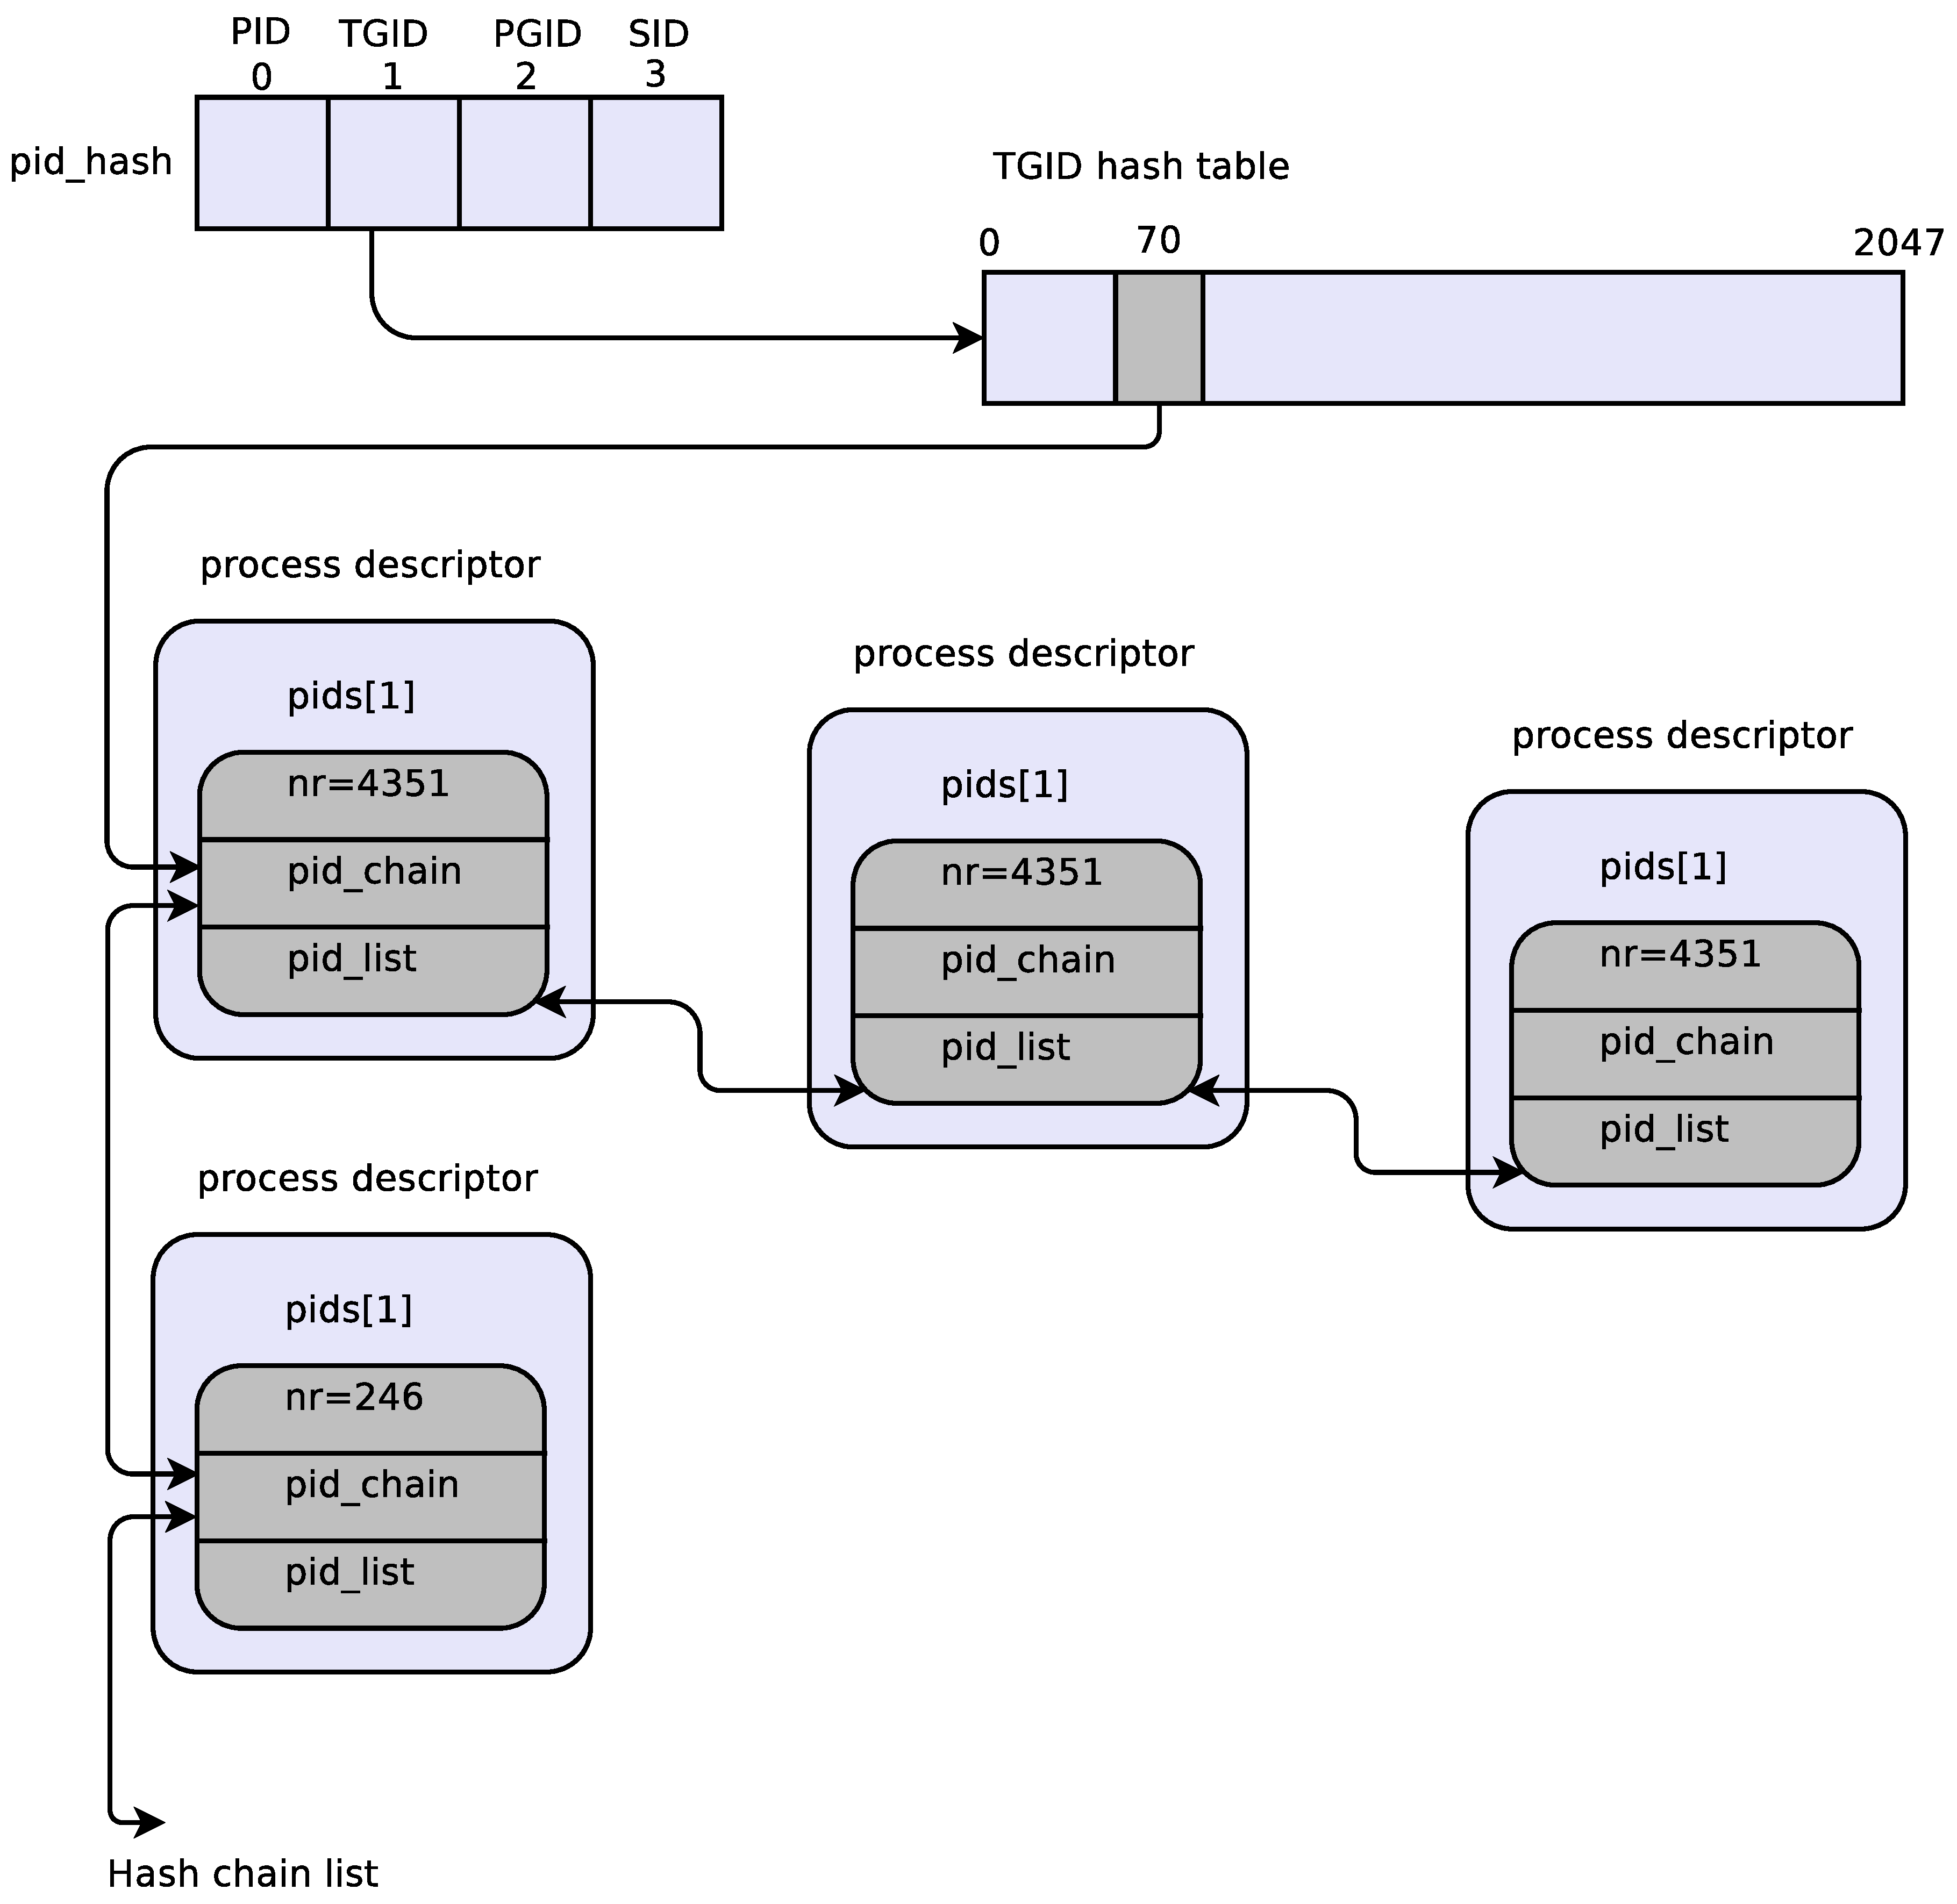
\includegraphics[width=.8\textwidth]{pidhashtable} }
    \mode<article>{ 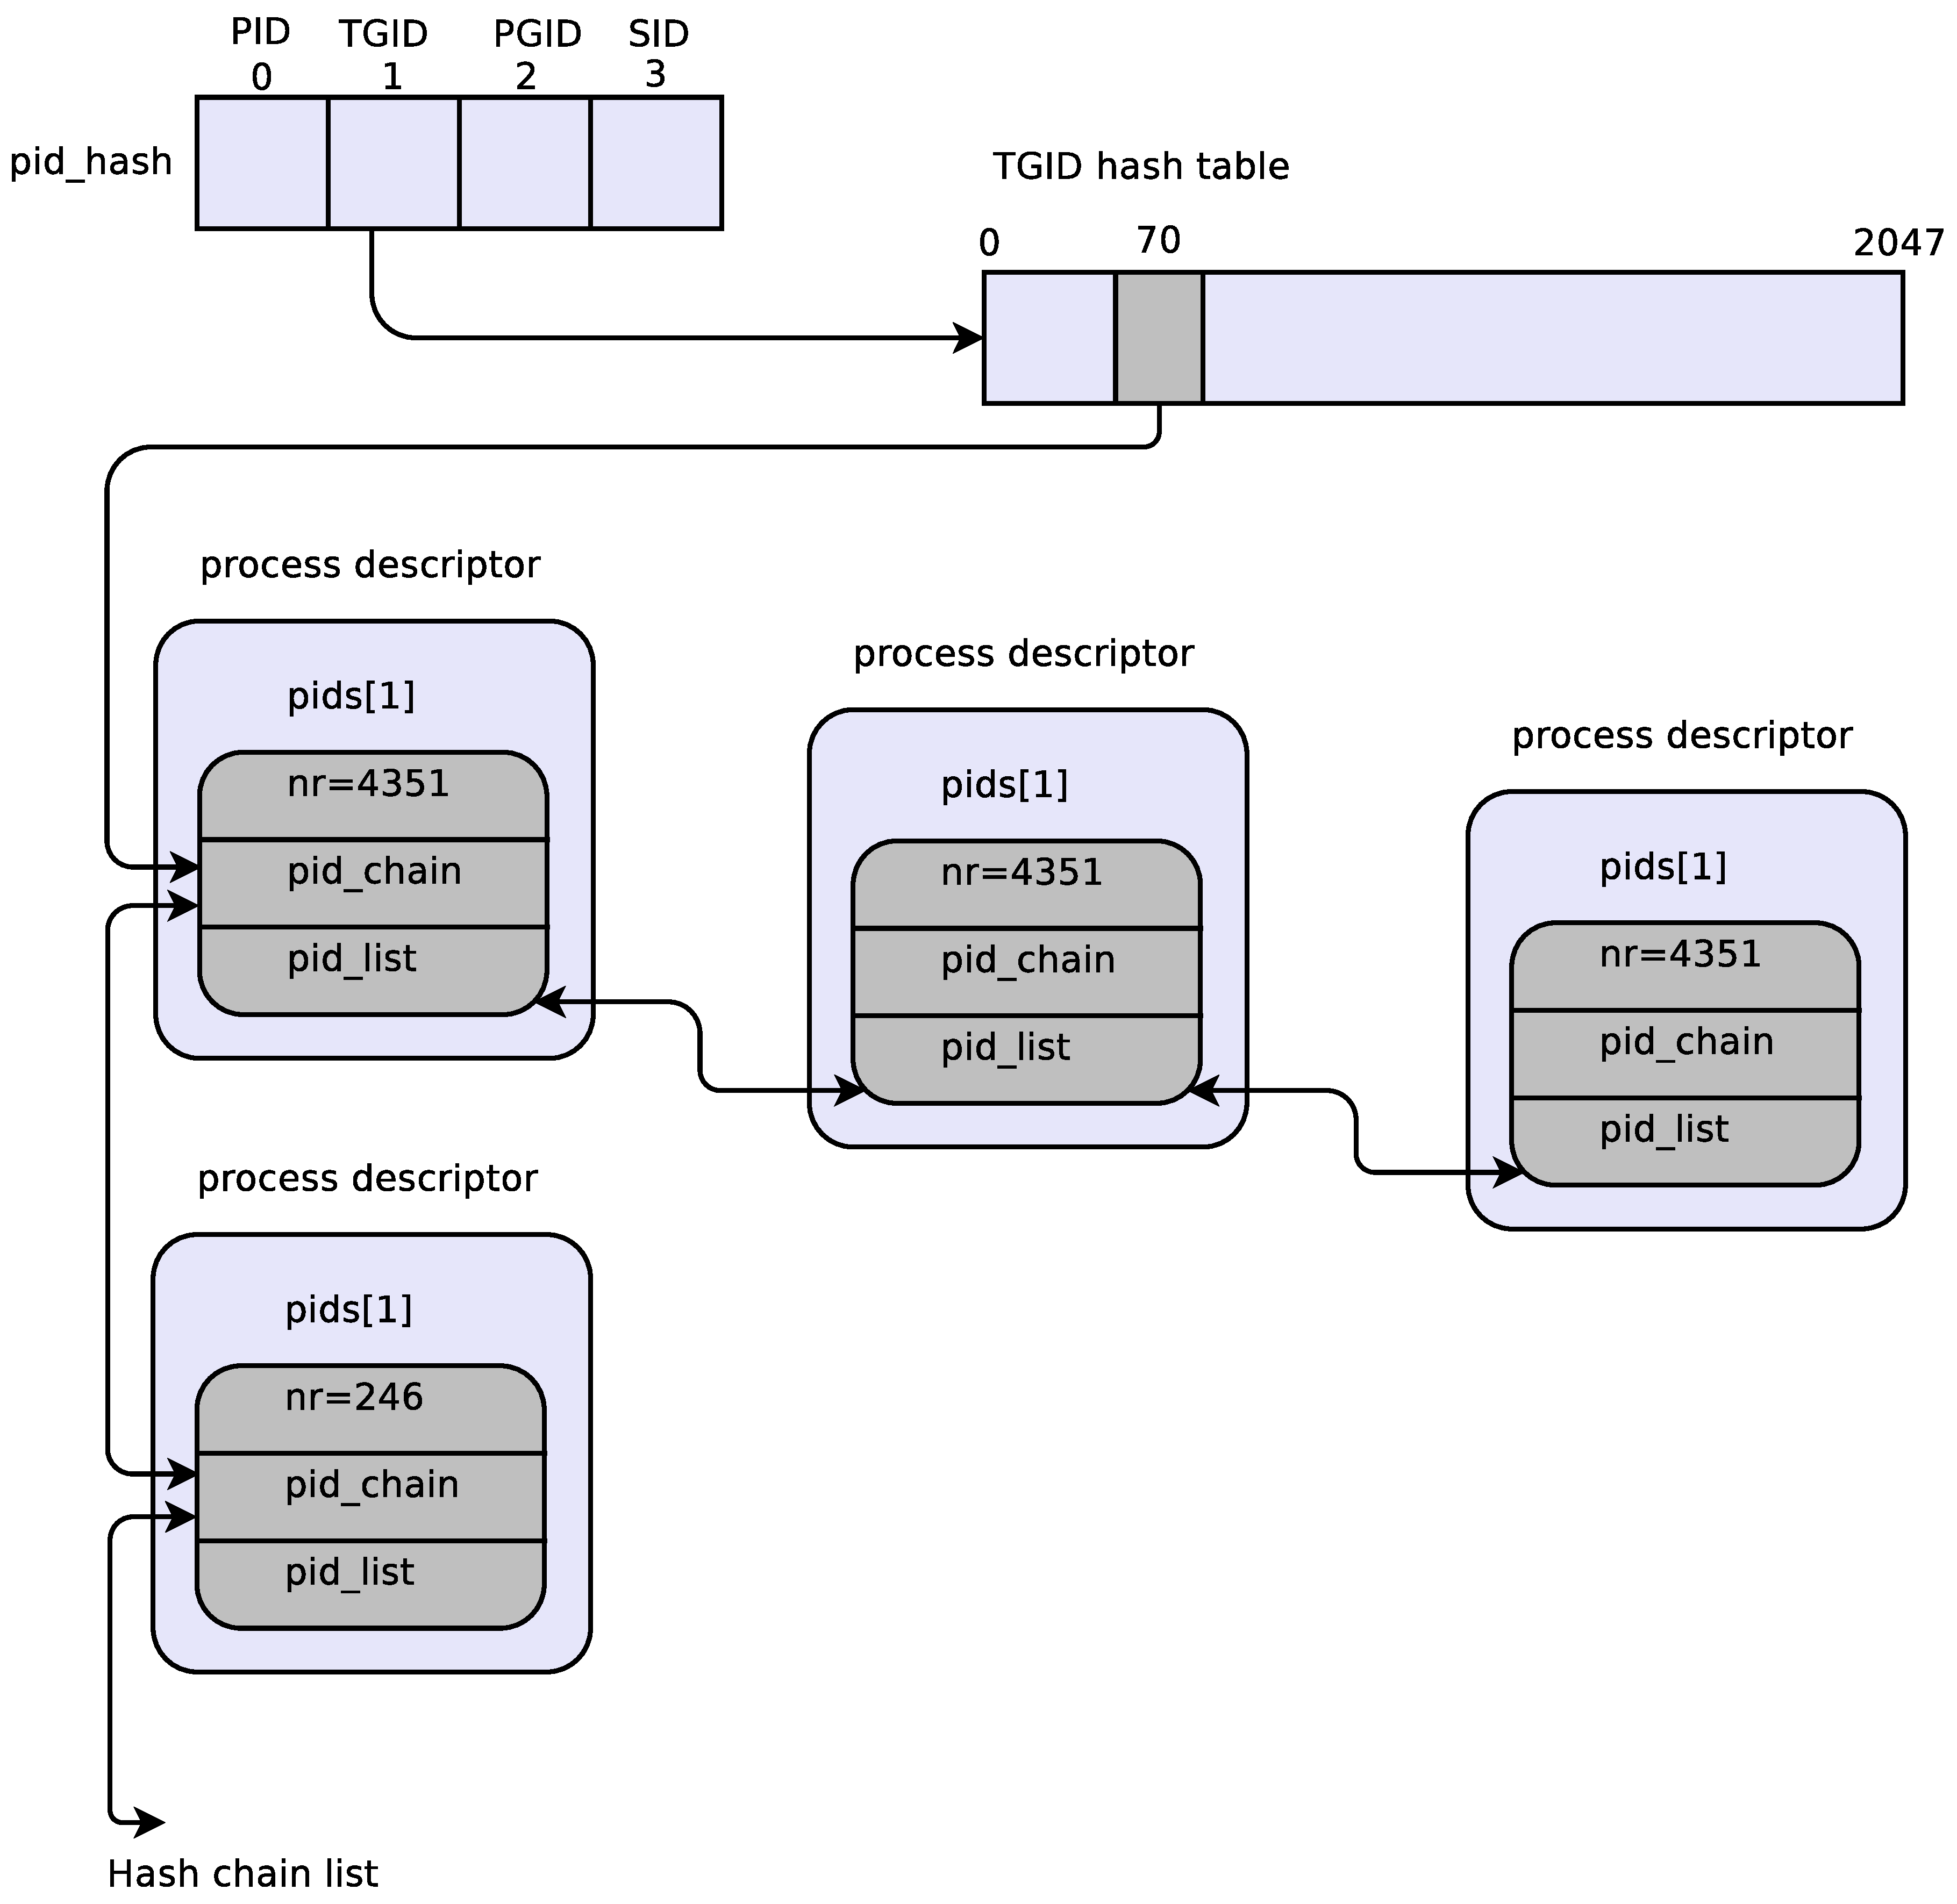
\includegraphics[width=.6\textwidth]{pidhashtable} }
  \end{center}
\end{frame}

\begin{frame}[fragile=singleslide]
  \begin{block}{\texttt{kernel/pid.c} --- Operations}
    \begin{itemize}
    \item \mintinline{c}{do_each_task_pid(nr, type, task)}
    \item \mintinline{c}{while_each_task_pid(nr, type, task)}
    \item \mintinline{c}{find_task_by_pid_type(type, nr)}
    \item \mintinline{c}{find_task_by_pid(nr)}
    \item \mintinline{c}{attach_pid(task, type, nr)}
    \item \mintinline{c}{detach_pid(task, type)}
    \item \mintinline{c}{next_thread(task)}
    \end{itemize}
  \end{block}
\end{frame}

\subsubsection{How Processes Are Organized}

\begin{frame}{Wait Queues}
  \begin{itemize}
  \item A wait queue represents a set of sleeping processes, which are woken up by the
    kernel when some condition becomes true.
  \item Wait queues are implemented as doubly linked lists whose elements include pointers
    to process descriptors.
  \end{itemize}
  \begin{block}{Each wait queue is identified by a \texttt{\_\_wait\_queue\_head}}
    \begin{center}
      \mode<beamer>{ \includegraphics[width=.8\textwidth]{wait1} }
      \mode<article>{ \includegraphics[width=.6\textwidth]{wait1} }
    \end{center}
    \begin{description}
    \item[lock:] avoid concurrent accesses.
    \end{description}
  \end{block}
\end{frame}

\begin{frame}
  \begin{block}{Elements of a wait queue list are of type \texttt{wait\_queue\_t}:}
    \begin{center}
      \mode<beamer>{ \includegraphics[width=.9\textwidth]{wait2} }
      \mode<article>{ \includegraphics[width=.5\textwidth]{wait2} }
    \end{center}
    \begin{description}
    \item[\texttt{task}:] address of this sleeping process
    \item[\texttt{task\_list}:] which wait queue are you in?
    \item[\texttt{flags}:] 1 -- exclusive; 0 -- nonexclusive;
    \item[\texttt{func}:] how it should be woken up?
    \end{description}
  \end{block}
\end{frame}

% \begin{frame}{Handling Wait Queues}{}
%   \begin{itemize}
%   \item DECLARE\_WAIT\_QUEUE\_HEAD(name) --- to define a new wait queue
%   \item init\_waitqueue\_head( ) --- to initialize a wait queue head variable
%   \item 
%   \end{itemize}
% \end{frame}

\subsubsection{Process Resource Limits}

\begin{frame}\mode<beamer>{\frametitle{Process Resource Limits}}
  \begin{block}{Limiting the resource use of a process}
    \begin{itemize}
    \item The amount of system resources a process can use are stored in the
      \texttt{current->signal->rlim} field.
    \item \texttt{rlim} is an array of elements of type \texttt{struct rlimit}, one for each
      resource limit.
    \end{itemize}
  \end{block}
  \begin{center}
    \mode<beamer>{ \includegraphics[width=.7\textwidth]{rlimit} }
    \mode<article>{ \includegraphics[width=.4\textwidth]{rlimit} }
  \end{center}
  \begin{description}
  \item[\texttt{rlim\_cur}:] the current resource limit for the resource
    \begin{itemize}
    \item[e.g.] \texttt{current->signal->rlim[RLIMIT\_CPU].rlim\_cur} --- the
      current limit on the CPU time of the running process.
    \end{itemize}
  \item[\texttt{rlim\_max}:] the maximum allowed value for the resource limit
  \end{description}
\end{frame}

\begin{frame}{Resource Limits}
  \begin{center}
    \begin{scriptsize}{\ttfamily
      \begin{tabular}{l|p{.7\textwidth}}
        RLIMIT\_AS&The maximum size of process address space\\\hline
        RLIMIT\_CORE&The maximum core dump file size\\\hline
        RLIMIT\_CPU&The maximum CPU time for the process\\\hline
        RLIMIT\_DATA&The maximum heap size\\\hline
        RLIMIT\_FSIZE&The maximum file size allowed\\\hline
        RLIMIT\_LOCKS&Maximum number of file locks\\\hline
        RLIMIT\_MEMLOCK&The maximum size of nonswappable memory\\\hline
        RLIMIT\_MSGQUEUE&Maximum number of bytes in POSIX message queues\\\hline
        RLIMIT\_NOFILE&The maximum number of open file descriptors\\\hline
        RLIMIT\_NPROC&The maximum number of processes of the user\\\hline
        RLIMIT\_RSS&The maximum number of page frames owned by the process\\\hline
        RLIMIT\_SIGPENDING&The maximum number of pending signals for the process\\\hline
        RLIMIT\_STACK&The maximum stack size
      \end{tabular}}
    \end{scriptsize}
  \end{center}
\end{frame}

\subsection{Process Switch}

\begin{frame}\mode<beamer>{\frametitle{Process Switch}}
  \begin{description}
  \item[Process execution context:] all information needed for the process execution
  \item[Hardware context:] the set of registers used by a process
  \end{description}
  \begin{block}{Where is the hardware context stored?}
    \begin{itemize}
    \item partly in the process descriptor (PCB)
    \item partly in the Kernel Mode stack
    \end{itemize}
  \end{block}
  \begin{block}{Process switch}
    \begin{itemize}
    \item saving the hardware context of {\texttt{prev}}
    \item replacing it with the hardware context of {\texttt{next}}
    \end{itemize}
  \end{block}
  \textcolor{blue}{Process switching occurs only in Kernel Mode.}
\end{frame}

\begin{frame}
  \begin{block}{Task State Segment (TSS)}
    \begin{itemize}
    \item For storing hardware contexts
    \item One TSS for each process (Intel's design)
    \item Hardware context switching
      \begin{itemize}
      \item {\texttt{far jmp}} to the TSS of {\texttt{next}}
      \end{itemize}
    \end{itemize}
  \end{block}
  \begin{block}{Linux doesn't use hardware context switch}
    \begin{itemize}
    \item One TSS for each CPU
      \begin{itemize}
      \item The address of the kernel mode stack
      \item I/O permission bitmap
      \end{itemize}
    \end{itemize}
  \end{block}
\end{frame}

\begin{frame}
  \begin{block}{Task State Segment Descriptor (TSSD)}
    \begin{center}
      \mode<beamer>{ \includegraphics[width=\textwidth]{tssd-anno} }
      \mode<article>{ \includegraphics[width=.6\textwidth]{tssd-anno} }
    \end{center}
    \begin{itemize}
    \item \texttt{S} bit set to 0;
    \item \texttt{Type} bits set to 9/11;
    \item \texttt{Busy} bit set to 1.
    \end{itemize}
  \end{block}
\end{frame}

\begin{frame}{The Task Register (\texttt{tr})}
  \begin{center}
    \mode<beamer>{ \includegraphics[width=.7\textwidth]{gdt-tss} }
    \mode<article>{ \includegraphics[width=.5\textwidth]{gdt-tss} }
  \end{center}
\end{frame}

\begin{frame}
  \begin{block}{Where to save the hardware context?}
    \begin{center}
      \mode<beamer>{ \includegraphics[width=.5\textwidth]{thread-struct} }
      \mode<article>{ \includegraphics[width=.3\textwidth]{thread-struct} }
    \end{center}
    \begin{itemize}
    \item \texttt{thread\_struct} includes fields for most of the CPU registers, except the
      general-purpose registers such as \texttt{eax, ebx}, etc., which are stored in
      the Kernel Mode stack.
    \end{itemize}
  \end{block}
\end{frame}

\begin{frame}{Performing The Process Switch}{\texttt{schedule()}}
  \begin{block}{Two steps:}
    \begin{enumerate}
    \item Switching the Page Global Directory
    \item Switching the Kernel Mode stack and the hardware context
    \end{enumerate}
  \end{block}
  \begin{block}{\texttt{switch\_to(prev,next,last)}}
    \begin{itemize}
    \item in any process switch three processes are involved, not just two
    \end{itemize}
  \end{block}
\end{frame}

\href{http://stackoverflow.com/questions/6525905/how-does-scheduleswitch-to-functions-from-linux-kernel-actually-work}{Stackoverflow:
  \textbf{How does \texttt{schedule()} + \texttt{switch\_to()} actually work?}}
\begin{itemize}
\item When a process runs out of time-slice, the flag \texttt{TIF\_NEED\_RESCHED} is set by
  \texttt{scheduler\_tick()}. (\href{http://http://lxr.linux.no/linux+v2.6.11/arch/i386/}{
    Called from the timer interrupt handler}, \texttt{set\_tsk\_need\_resched()})
\item The kernel checks the flag, sees that it is set, and calls \texttt{schedule()} to
  switch to a new process. This flag is a message that schedule should be invoked as soon
  as possible because another process deserves to run. Upon returning to user-space or
  returning from an interrupt, the \texttt{TIF\_NEED\_RESCHED} flag is checked. If it is
  set, the kernel invokes the scheduler before continuing.
\end{itemize}

  
\subsection{Creating Processes}

\begin{itemize}
\item \citetitle[Chapter 2, \emph{Process Management And Scheduling}]{mauerer2008professional}
\item \citetitle[Section 3.3. \emph{Process Creation: fork(), vfork(), and clone() System
    Calls}]{rodriguez2005linux}
\item \citetitle[Section 3.2, \emph{Process Creation}]{love2010linux}
\end{itemize}

\begin{frame}[fragile=singleslide]{Creating Processes}
  \begin{block}{The \texttt{clone()} system call}
    \begin{center}
      \mode<beamer>{ \includegraphics[width=\textwidth]{clone1} }
      \mode<article>{ \includegraphics[width=.6\textwidth]{clone1} }
    \end{center}
  \end{block}
  \begin{block}{The traditional \texttt{fork()} system call}
    \mintinline{c}{clone(func, child_stack, SIGCHLD, NULL);}
    \begin{itemize}
    \item \texttt{child\_stack}: parent stack pointer (copy-on-write)
    \end{itemize}
  \end{block}
  \begin{block}{\texttt{vfork()}}
    \mintinline{c}{clone(func, child_stack, CLONE_VM|CLONE_VFORK|SIGCHLD, NULL);}
    \begin{itemize}
    \item \texttt{child\_stack}: parent stack pointer (copy-on-write)
    \end{itemize}
  \end{block}
\end{frame}

\begin{frame}
  \begin{block}{The \texttt{do\_fork()} function does the real work}
    \begin{center}
      \mode<beamer>{ \includegraphics[width=.7\textwidth]{syscall} }
      \mode<article>{ \includegraphics[width=.4\textwidth]{syscall} }
    \end{center}
  \end{block}
\end{frame}

\begin{frame}
  \begin{block}{\texttt{do\_fork()} calls \texttt{copy\_process()} to make a copy of
      process descriptor}
    \begin{center}
      \mode<beamer>{ \includegraphics[width=.8\textwidth]{do-fork} }
      \mode<article>{ \includegraphics[width=.6\textwidth]{do-fork} }
    \end{center}
  \end{block}
\end{frame}

\begin{frame}
  \begin{block}{\texttt{copy\_process()}}
    \begin{enumerate}
    \item \texttt{dup\_task\_struct()}: creates
      \begin{itemize}
      \item a new kernel mode stack
      \item \texttt{thread\_info}
      \item \texttt{task\_struct}
      \end{itemize}
      Values are identical to the parent
    \item is \texttt{current->signal->rlim[RLIMIT\_NPROC].rlim\_cur} confirmed?
    \item Update child's \texttt{task\_struct}
    \item Set child's state to \texttt{TASK\_UNINTERRUPTABLE}
    \item \texttt{copy\_flags()}: update flags in \texttt{task\_struct}
     \item \texttt{get\_pid()} (check \texttt{pidmap\_array} bitmap)
    \item Duplicate or share resources (opened files, FS info, signal, ...)
    \item \texttt{return p;}
    \end{enumerate}
  \end{block}
\end{frame}

See also: \citetitle[Sec~3.2.2, \emph{Forking}]{love2010linux}

\begin{frame}{Creating A Kernel Thread}
  \begin{block}{\texttt{kernel\_thread()} is similar to \texttt{clone()}}
    \begin{center}
      \mode<beamer>{ \includegraphics[width=.9\textwidth]{kernel-thread} }
      \mode<article>{ \includegraphics[width=.8\textwidth]{kernel-thread} }
    \end{center}
  \end{block}
\end{frame}

\begin{itemize}
\item Typically, a kernel thread continues executing its initial function forever (or at
  least until the system reboots, but with Linux you never know). The initial function
  usually implements a loop in which the kernel thread wakes up as needed, performs its
  duties, and then returns to sleep \citetitle[Sec 3.4.2, \emph{Kernel Threads}]{love2010linux}.
\end{itemize}

\begin{frame}{Process 0}
  \begin{description}
  \item[Process 0] is a kernel thread created from scratch during the initialization
    phase.
    \begin{itemize}
    \item Also called \emph{idle process}, or \emph{swapper process}
    \item Its data structures are \emph{statically} allocated
    \end{itemize}
  \end{description}
  \begin{block}{\texttt{start\_kernel()}}
    \begin{itemize}
    \item Initializes all the data structures
    \item Enables interrupts
    \item Creates another kernel thread --- \emph{process 1, the \texttt{init} process}
    \end{itemize}
  \end{block}
\end{frame}

\begin{frame}
  \begin{block}{Call graph}
    \begin{center}
      \mode<beamer>{ \includegraphics[width=.9\textwidth]{start-kernel} }
      \mode<article>{ \includegraphics[width=.7\textwidth]{start-kernel} }
    \end{center}
  \end{block}
  \begin{itemize}
  \item After having created the \emph{init} process, \emph{process 0} executes the
    \texttt{cpu\_idle()} function.
  \item Process 0 is selected by the scheduler only when there are no other processes in
    the \texttt{TASK\_RUNNING} state.
  \item In multiprocessor systems there is a process 0 for each CPU.
  \end{itemize}
\end{frame}

\begin{frame}{Process 1}
  \begin{itemize}
  \item Created via \mbox{{\small \texttt{kernel\_thread(init, NULL, CLONE\_FS|CLONE\_SIGHAND);}}}
  \item \texttt{PID} is 1
  \item shares all per-process kernel data structures with process 0
  \item starts executing the \texttt{init()} function
    \begin{itemize}
    \item completes the initialization of the kernel
    \end{itemize}
  \item \texttt{init()} invokes the \texttt{execve()} system call to load the executable
    program \texttt{init}
    \begin{itemize}
    \item As a result, the \emph{init kernel thread} becomes a regular process having its
      own per-process kernel data structure
    \end{itemize}
  \item The init process stays alive until the system is shut down
  \end{itemize}
\end{frame}

\subsection{Destroying Processes}

\begin{frame}{Process Termination}
  \begin{itemize}
  \item Usual way: call \texttt{exit()}
    \begin{itemize}
    \item The C compiler places a call to \texttt{exit()} at the end of \texttt{main()}.
    \end{itemize}
  \item Unusual way: \texttt{Ctrl-C ...}
  \end{itemize}
\end{frame}

\begin{frame}
  \begin{block}{All process terminations are handled by \texttt{do\_exit()}}
    \begin{itemize}
    \item \texttt{tsk->flags |= PF\_EXITING;} to indicate that the process is being eliminated
    \item \texttt{del\_timer\_sync(\&tsk->real\_timer);} to remove any kernel timers
    \item \texttt{exit\_mm(), exit\_sem(), \_\_exit\_files(), \_\_exit\_fs(),
        exit\_namespace(), exit\_thread()}: free pointers to the kernel data structures
    \item \texttt{tsk->exit\_code = code;}
    \item \texttt{exit\_notify()} to send signals to the task's parent
      \begin{itemize}
      \item re-parents its children
      \item sets the task's state to \texttt{TASK\_ZOMBIE}
      \end{itemize}
    \item \texttt{schedule()} to switch to a new process
    \end{itemize}
  \end{block}
\end{frame}

\begin{frame}{Process Removal}
  Cleaning up after a process and removing its process descriptor are separate.
  \begin{block}{Clean up}
    \begin{itemize}
    \item done in \texttt{do\_exit()}
    \item leaves a zombie
      \begin{itemize}
      \item To provide information to its parent
      \item The only memory it occupies is its kernel stack, the \texttt{thread\_info}
        structure, and the \texttt{task\_struct} structure.
      \end{itemize}
    \end{itemize}
  \end{block}
\end{frame}

\begin{frame}
  \begin{block}{Removal}
    \begin{itemize}
    \item \texttt{release\_task()} is invoked by
      \begin{itemize}
      \item[either] \texttt{do\_exit()} if the parent didn't wait
      \item[or] \texttt{wait4()/waitpid()}
      \end{itemize}
    \item \texttt{free\_uid()}
    \item \texttt{unhash\_process}: to remove the process from the pidhash and from the task
      list
    \item \texttt{put\_task\_struct()}
      \begin{itemize}
      \item free the pages containing the process's kernel stack and \texttt{thread\_info}
        structure
      \item de-allocate the slab cache containing the \texttt{task\_struct}
      \end{itemize}
    \end{itemize}
  \end{block}
\end{frame}

\mode<all>
%%% Local Variables:
%%% mode: latex
%%% TeX-master: "kernel-b"
%%% End:
